\section{Checkpoint 3}

\addtocounter{subsection}{1}

\subsection{What is a Programm? What is a Process? What is a Thread?}
Ein Programm ist eine ausf\"uhrbare Datei.\\
Ein Prozess ist ein laufendes Programm.\\
Ein Thread ist ein Ausf\"uhrungsstrang eines Programms.

\subsection{What are the roles of the scheduler and the dispatcher?}
Der Scheduler hat die Aufgabe den laufenden Prozessen ihre CPU Zeit zuzuweisen.\\
Der Dispatcher gibt die Kontrolle zum dem n\"achsten aktiven Thread(wiederherstellen des CPU Kontextes, vorbereiten des Adressbereiches f\"ur den n\"achsten Prozess).

\subsection{Compare the long term scheduler to the short term scheduler.}
Long-term scheduler(Steuert Grad der Multiprogrammierung, kann Prozesse schlafen legen, optional)\\
Short-term scheduler(Sucht zu jedem Quantum einen neuen Thread aus, Scheduler \"uber den wir immer reden)

\subsection{Describe 3 properties related to process and thread control objects.}
\begin{itemize}
	\setlength\itemsep{-0.5em}
	\item Prozess: Speicherbereich, Pfad der ausf\"uhrbaren Datei
	\item Thread: CPU Kontext, Schedulingzustand
	\item Beides: Nicewert(Priorit\"aten), ID
\end{itemize}

\subsection{Describe 3 properties related to the CPU context.}
Prozessorstatuswort, Stackregister, Datenregister, Programmcounter

\subsection{Outline the sequence of a context switch as performed by the dispatcher.}
Aktuellen Thread unterbrechen $\rightarrow$ Aktuellen Zustand sichern im Hauptspeicher $\rightarrow$ Daten vom anderen Thread zur\"uckschreiben $\rightarrow$ anderen Thread ausf\"uhren

\subsection{Compare cooperative to preemptive scheduling.}
\textbf{cooperative} freiwillige Abgabe der CPU\\
\textbf{preemptive} Unterbrechung, wenn Quantum abgelaufen

\subsection{What is a quantum? What effect does the length of a quantum have on the scheduler performance?}
Ein Quantum ist eine feste Zeitscheibe, welche angibt wie lange ein Prozess rechnen darf, bis er unterbrochen wird. L\"angeres Quantum sorgt f\"ur eine h\"ohere Performanz. K\"urzeres Quantum ist responsiver.

\subsection{Threads can have different states in relation to scheduling. Draw a diagram and Describe the purpose of the states and their transitions.}

\begin{figure}[H]
	\centering
	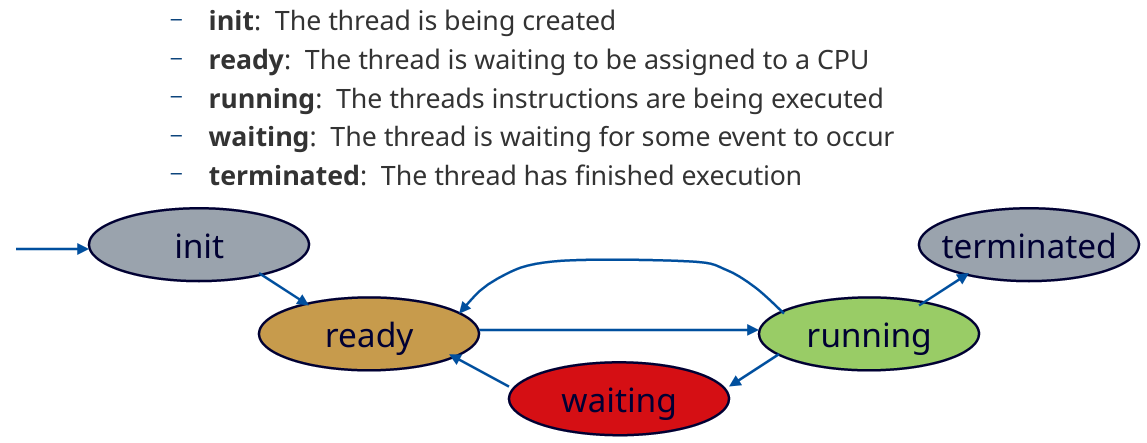
\includegraphics[width=0.7\linewidth]{Pictures/scheduling_dia}
\end{figure}

\subsection{When are scheduling decisions made?}
Am Ende von jedem Quantum. Welcher Thread als n\"achstes in \textbf{running} darf. Immer wenn ein neuer thread im system ankommt.

\subsection{What are the optimiztion criteria of a scheduler?}
\begin{itemize}
	\setlength\itemsep{-0.5em}
	\item Resposivit\"at
	\item Durchsatz
	\item Wartezeit
	\item Turn Arount Time(Zeit vom ersten Ausf\"uhren eines Threads bis zum letzten Ausf\"uhren)
	\item Auslast der CPU 
\end{itemize}

\subsection{Draw a FIFO Gantt Chart for the given taskset. Assume a context switch takes no time.}
\begin{figure}[H]
	\centering
	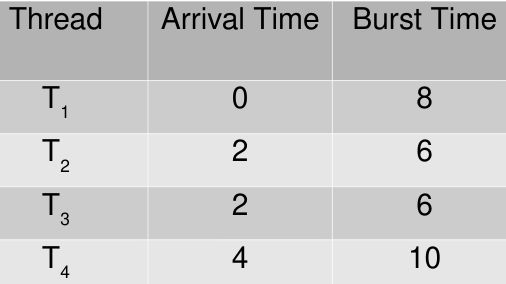
\includegraphics[width=0.25\linewidth]{Pictures/scheduling_gantt_table_fifo}
\end{figure}
\begin{figure}[H]
	\centering
	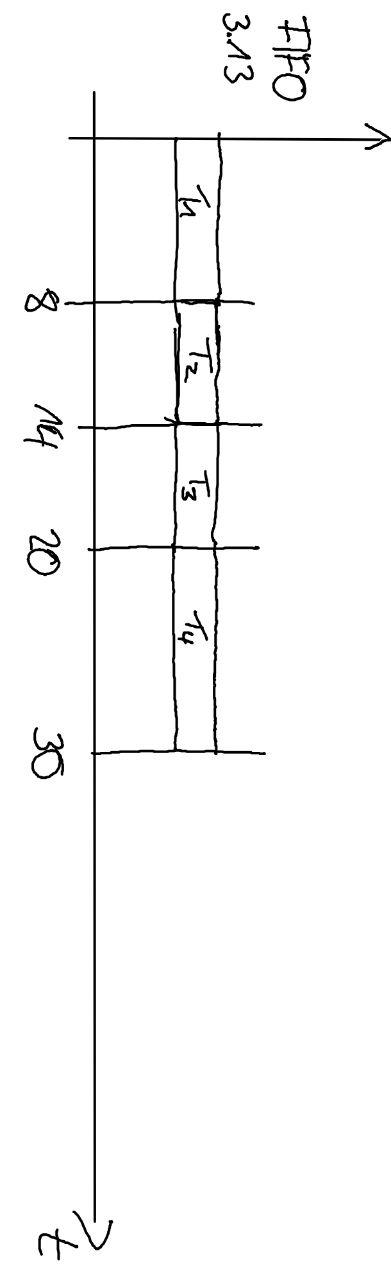
\includegraphics[width=0.25\linewidth,angle=90,origin=c]{Pictures/scheduling_gantt_dia_fifo}
\end{figure}

\subsection{Draw a Round Robin Gantt chart for the given taskset. Assume a context switch takes not time, use quantum of length 3}
\begin{figure}[H]
	\centering
	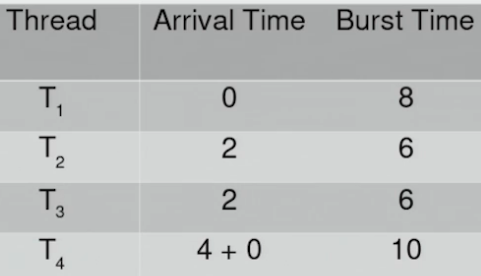
\includegraphics[width=0.25\linewidth]{Pictures/scheduling_gantt_table_rr}
\end{figure}
\begin{figure}[H]
	\centering
 	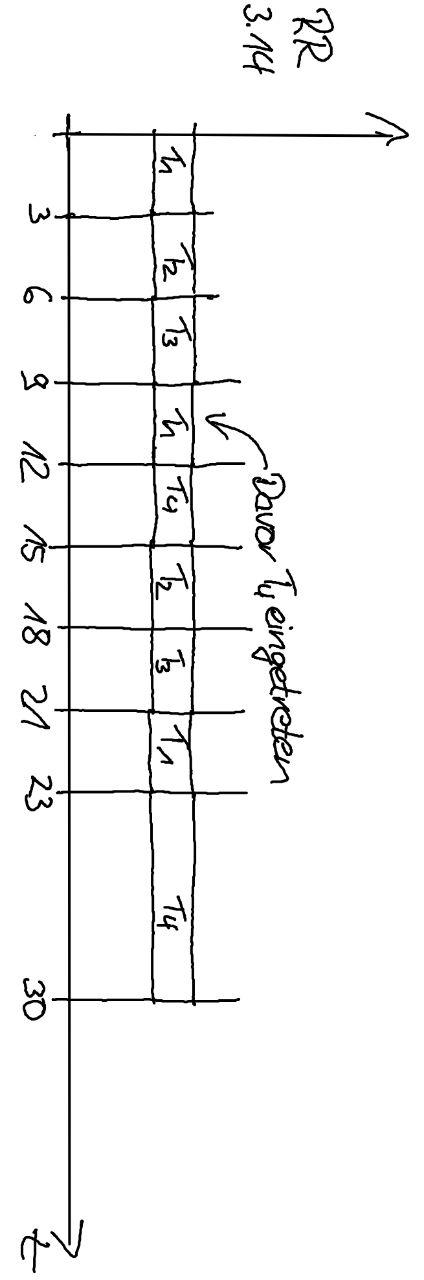
\includegraphics[width=0.25\linewidth,angle=90,origin=c]{Pictures/scheduling_gantt_dia_rr}
\end{figure}

\subsection{Draw a Round Robin Gantt chart for the given taskset. Assume a context switch takes not time, use quantum of length 3}
\begin{figure}[H]
	\centering
	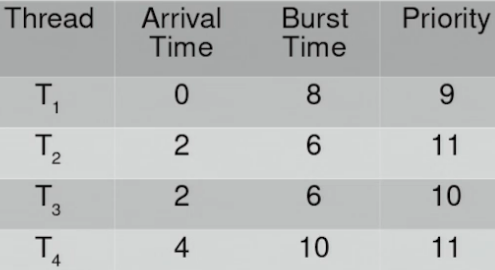
\includegraphics[width=0.25\linewidth]{Pictures/scheduling_gantt_table_rr_prio}
\end{figure}
\begin{figure}[H]
	\centering
	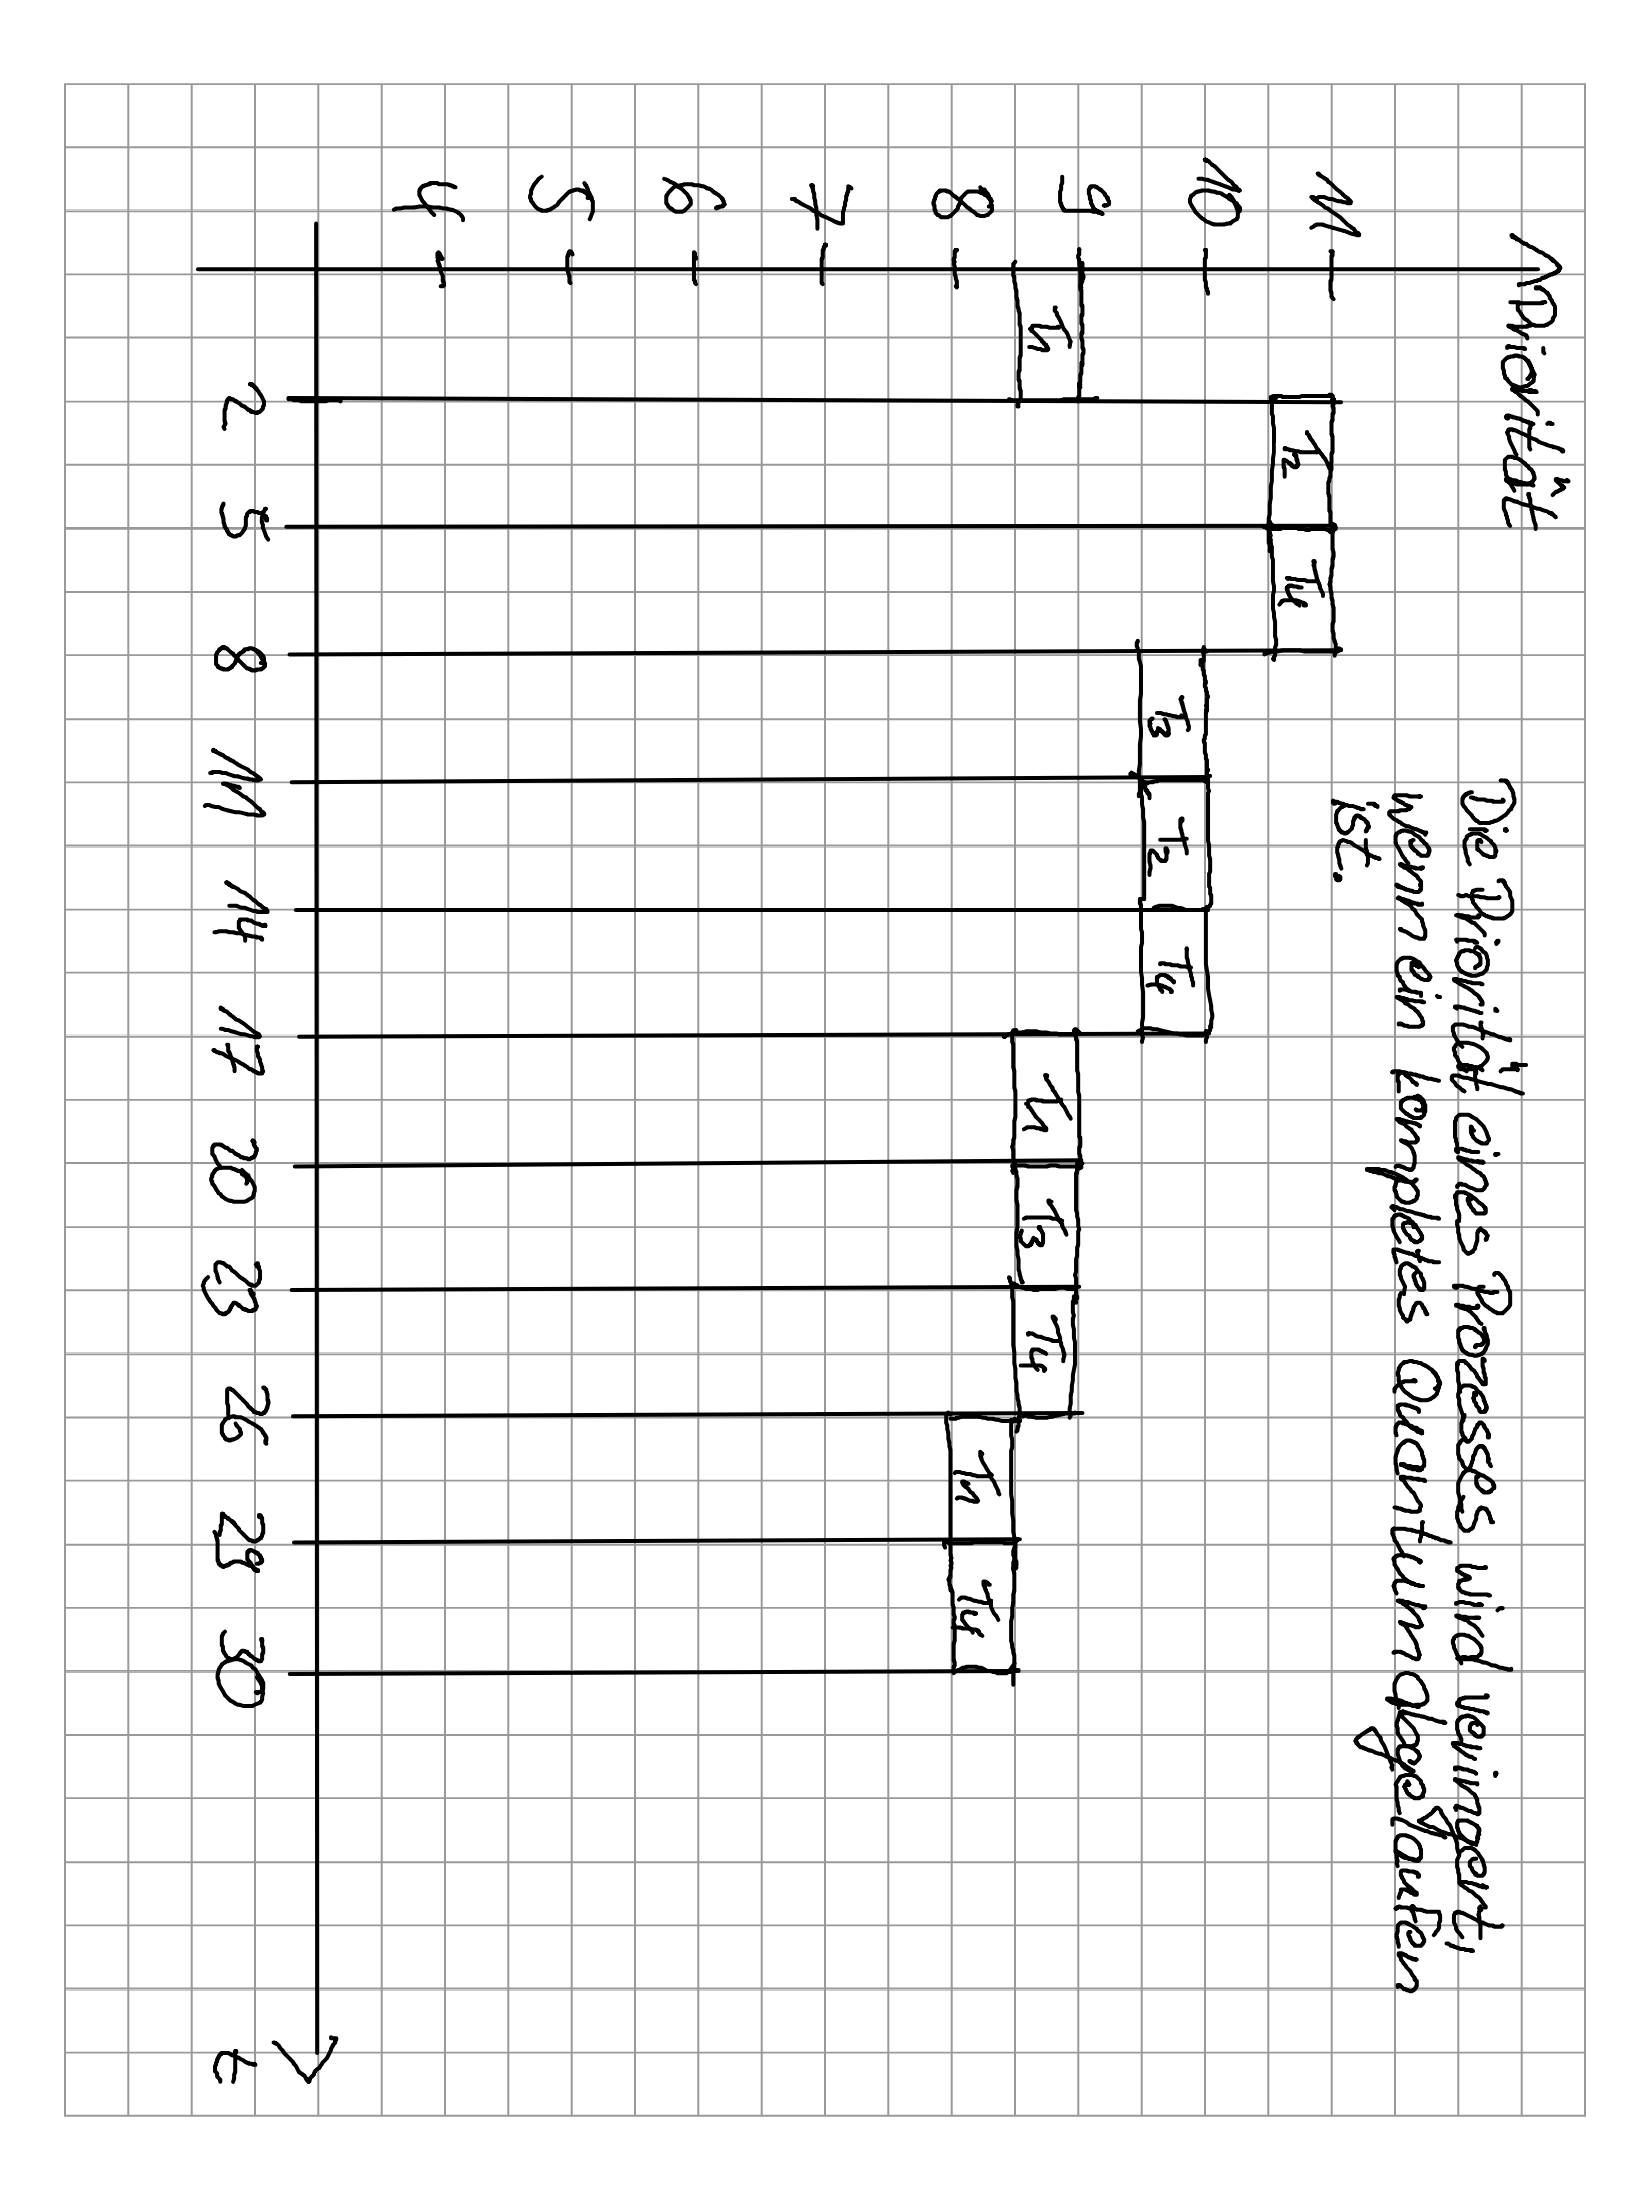
\includegraphics[width=0.6\linewidth,angle=90,origin=c]{Pictures/scheduling_gantt_dia_rr_prio}
\end{figure}

\subsection{Calculate for each thread waiting time, turnaround time, throughput and compare}
\begin{itemize}
	\setlength\itemsep{-0.5em}
	\item \textbf{waiting time} eintreten in die Queue bis zur Ausf\"uhrung der ersten Instruktion
	\item $Time Of First Instruction - ArrivalTime = WaitingTime$
	\begin{multicols}{3}
	\item FIFO
	\begin{itemize}
		\item $T_1=0$
		\item $T_2=8-2=6$
		\item $T_3 = 14-2=12$
		\item $T_4 = 20-4=16$
	\end{itemize}
	\columnbreak
	\item RR
	\begin{itemize}
		\item $T_1 = 0$
		\item $T_2 = 3-2=1$
		\item $T_3 = 6-2=4$
		\item $T_4 = 12-4=8$
	\end{itemize}
	\columnbreak
	\item RR + Prio
	\begin{itemize}
		\item $T_1 = 0$
		\item $T_2 = 0$
		\item $T_3 = 8-2=6$
		\item $T_4 = 5-4=1$
	\end{itemize}
	\end{multicols}
	\item	\textbf{Turn Around Time} Zeit die der Task im System verbringt
	\begin{multicols}{3}
		\item FIFO
		\begin{itemize}
			\item $T_1= Burst = 8$
			\item $T_2=Burst=6$
			\item $T_3 =Burst=6$
			\item $T_4 =Burst=10$
		\end{itemize}
		\columnbreak
		\item RR
		\begin{itemize}
			\item $T_1 = 23$
			\item $T_2 = 18-3=15$
			\item $T_3 = 21-6=15$
			\item $T_4 = 30-12=18$
		\end{itemize}
		\columnbreak
		\item RR + Prio
		\begin{itemize}
			\item $T_1 = 29$
			\item $T_2 = 14-2=12$
			\item $T_3 = 23-8=15$
			\item $T_4 = 30-5=25$
		\end{itemize}
	\end{multicols}
	\item \textbf{response time} Eintritt in die Warteschlange bis zur erste Antwort des BS.
	\item \textbf{throuput} Menge der Threads pro Zeiteinheit. Hier: 4 Threads/30 Zeiteinheiten(auf Grund der Annahme, Kontextwechsel==0 !)
\end{itemize}

\subsection{Describe the problem of thread starvation in relation to priority schedulers.}
Ein Thread mit hoher Priorit\"at h\"alt einen Thread mit niedriger Priorit\"at vom laufen ab.

\subsection{What is a multilevel queue scheduler? Linux and Windows both contain multilevel queue schedulers. Name an example for a queue level and describe what properties threads in this queue have.}
Scheduler der mehrere queues hat. In einander verschachtelt.\\
Windows: 16 Prios + 16 Realtime Prios (Algorithmen)\\
Linux: FIFO, RR + Batch, Idle\\
\missing\\
\unsure

\subsection{Name 2 functions related to process or thread creation.}
Linux: PThreadcreate(), fork()\\Windows: CreateProcess(), CreateThread()
\subsubsection{Name 2 functions related to process or thread termination.}
Linux: exit(), pthreadexit()\\Windows: kill(), abort()

\subsection{Compare the Linux semantics of process creation (fork/exec) to the windows semantics of process creation (CreateProcess).}
Linux fork(), exec() habe ich 2 Funktionen in den ich Sachen machen kann.\\
Windows in CreateProcess kann ich keine Sachen machen und ich habe nur eine Funktion. Parameter\"ubergabe f\"ur Pipes als Argument integriert.

\subsection{What are the advantages and disadvantages of multithreading in a programm?}
Wir m\"ussen unsere geteilten Resourcen vor einander sch\"utzen. Wir k\"onnen eine h\"ohere Auslastung des Systems erreichen.

\subsection{Compare User Mode Threads to Kernel Mode Threads. When would you use which?}
Kernel Mode Threads sind Threads die wirklich auf Threads im Kernel abbilden. Umgekehrt f\"ur User Mode Threads.

\subsection{What are Fibers?}
\begin{itemize}
	\setlength\itemsep{-0.5em}
	\item[a:] User Mode Threads on Windows
	\item[b:] The Windows equivalent of UNIX pipes
	\item[c:] Units of time counted in the Linux Kernel
	\item[d:] Users in a traditional UNIX system
\end{itemize}
Antwort \textbf{A}

\subsection{What are cgroups?}
\begin{itemize}
	\setlength\itemsep{-0.5em}
	\item[a:] groups of capabilities of an executable
	\item[b:] groups of redundant file system entries
	\item[c:] isolated process control groups in Linux
	\item[d:] groups of users in Windows
\end{itemize}
Antwort \textbf{C}: Prozessgruppen die voneinander isoliert werden. Bsp. Docker

\subsection{Describe the specific challenges of real-time scheduling. What is the difference between soft and hard real-time?}
Software die mit Deadlines umgehen k\"onnen muss. Soft: Dienst degradiert Bsp. Youtube, Hard: Autokontrolle, Flugzeugkontrolle $\rightarrow$ Unfall, Katastrophe\\
Sehr schwierig, weil man kann die Verz\"ogerungen nicht im Vorraus kennen(Caches, Interrupts)

\subsection{Describe one of the three discussed approaches of starvation avoidance.}
PrioBoosting on Windows\\PrioAgeing, Niceness on Linux\\
PrioBoosting: Thread bekommt kurz eine sehr hohe Prio sinkt dann aber wieder ab\\
PrioAgeing: Threads werden St\"uck f\"ur St\"uck abgesenkt

\subsection{What is priority inversion?}
Thread mit niedriger Prio h\"alt Thread mit hoher Prio vom laufen ab $\rightarrow$ Locks\\

\begin{figure}[H]
	\centering
	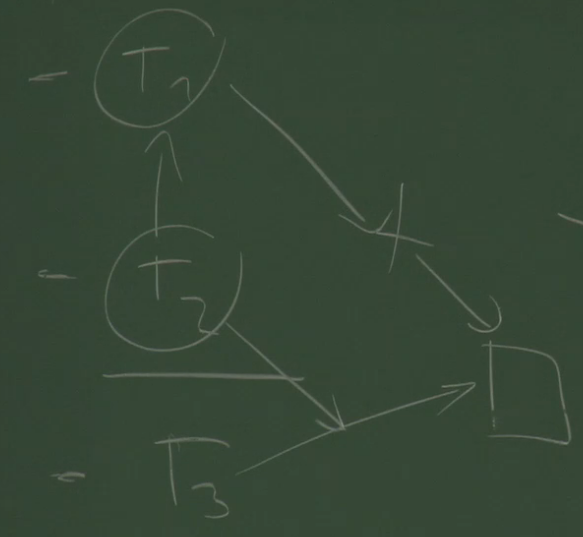
\includegraphics[width=0.5\linewidth]{Pictures/priority_inversion}
\end{figure}

\subsection{Which of the following is not a queue level in Completely Fair Scheduler (CFS)?}
\begin{itemize}
	\setlength\itemsep{-0.5em}
	\item[a:] SCHED\_BATCH
	\item[b:] SCHED\_HIGH
	\item[c:] SCHED\_RR
	\item[d:] SCHED\_FIFO
\end{itemize}
Antwort \textbf{b}: ist Ausgedacht von dem Dozenten

\subsection{Describe the concept of niceness in relation to the Linux Completely Fair Scheduler (CFS).}
Wir haben einen relativen Wert zwischen $\pm$20. Der Wert beschreibt das Verh\"altnis L\"ange der Ausf\"uhrungszeit, die die Threads zu einander bekommen mit einer Nicewert Differenz von ca 1,25 entsprechend der Laufzeit.\\Ein Thread der 1 niedrigeren Nicewert hat als ein anderer Thread, wird 1,25 mal so lange ran kommen.

\subsection{What is thread affinity? Compare hard affinity and soft affinity.}
Bitmaske, welche auf einem Multicore System festlegt auf welchen Core ich laufen darf. Ich darf auf den Kernen laufen, auf denen meine Affinit\"atsmaske eine 1 hat.\\
Bei harter Affinit\"at kann dies manuell eingestellt werden.\\
Bei softer Affinit\"at wird dem Thread zu erst der Core zugewiesen, welcher am besten ist. Beim Fortsetzen wird versucht wieder diesen Core zu benutzen da hier alle Daten schon vorhanden sind.

\subsection{On a high level, outline the similarities and differences of the Windows and Linux Scheduler.}
Gemeinsamkeiten: Priorit\"aten\\
Linux: Nicewerte\\
Windows: \\
$\dots$\\
\missing